% DOCUMENTO PRINCIPAL

% Este es el fichero principal de este repositorio. No se recomienda editarlo.
% Modifica las plantillas incluidas en los directorios:
% - secciones
% - tablas
% - algoritmos

\documentclass[final,a4paper,11pt,twoside]{class_diss}

\usepackage[full]{textcomp}
\usepackage{graphicx}
\usepackage{amsmath}
\usepackage{amsxtra}
\usepackage{amssymb}
\usepackage{amsthm}
\usepackage{latexsym}
\usepackage{setspace}
\usepackage[margin=3cm]{geometry}
\usepackage[titles]{tocloft}
\usepackage{latexsym}
\usepackage{fancyhdr}
\usepackage{emptypage}
\usepackage[svgnames,dvipsnames,usenames,table,xcdraw]{xcolor}
\usepackage{tikz}
\usepackage[toc,acronym,nonumberlist,xindy={language=spanish-traditional},sanitize=none]{glossaries}
\usepackage[scaled]{helvet}
\usepackage[utf8]{inputenc}
\usepackage[T1]{fontenc}
\usepackage[spanish,es-tabla]{babel}
\usepackage[explicit]{titlesec}
\usepackage{newtxtext}
\usepackage{newtxmath}
\usepackage{stmaryrd}
\usepackage{bbold}
\usepackage[ruled,vlined]{algorithm2e}
\usepackage{algorithmic}
\usepackage{float}
\usepackage{url}
\usepackage{xspace}
\usepackage{booktabs}
\usepackage{multirow}
\usepackage{enumitem}
\usepackage{rotating}
\usepackage{pdflscape}
\usepackage{listings}
\usepackage{placeins}
\usepackage{flafter}
\usepackage{pdfpages}

\usepackage{tcolorbox}
\tcbset {
  base/.style={
    arc=0mm, 
    bottomtitle=0.5mm,
    boxrule=0mm,
    colbacktitle=black!10!white, 
    coltitle=black, 
    fonttitle=\bfseries, 
    left=2.5mm,
    leftrule=1mm,
    right=3.5mm,
    title={#1},
    toptitle=0.75mm, 
  }
}

\definecolor{brandblue}{rgb}{0.34, 0.7, 1}
\newtcolorbox{mainbox}[1]{
  colframe=brandblue, 
  base={#1}
}

\newtcolorbox{subbox}[1]{
  colframe=black!30!white,
  base={#1}
}


\theoremstyle{definition}
\newtheorem{definition}{Teorema}[section]
\theoremstyle{remark}
\newtheorem*{remark}{Remark}
\DeclareMathOperator*{\argmax}{arg\,max}
\DeclareMathOperator*{\argmin}{arg\,min}
\definecolor{VIU}{RGB}{240, 90, 15}
\definecolor{DESTACADO}{RGB}{130, 34, 145}
\definecolor{CITA}{RGB}{0, 123, 194}

\renewcommand{\algorithmcfname}{Algoritmo}
\renewcommand{\acronymname}{Lista de Acr\'onimos}
\addto\captionsspanish{
    \renewcommand*{\acronymname}{Lista de Acr\'onimos}
}
\newcommand{\inhib}{\relbar\mapsfromchar}
\newcommand{\destacado}[1]{\color{DESTACADO}\textbf{#1}\color{black}\xspace}

\usetikzlibrary{shapes}
\newcommand*\circled[1]{\tikz[baseline=(char.base)]{
    \node[shape=diamond,fill=black!90,inner sep=1pt,minimum size=1cm] (char) {\textcolor{white}{\small\textbf{#1}}};}
}

\pagestyle{fancy}
\fancyhf{}
\fancyhead[LO]{}
\fancyhead[RE]{}
\fancyfoot[C]{}
\renewcommand{\headrulewidth}{0pt}

\fancypagestyle{plain}{
  \fancyhf{}
  \fancyfoot[C]{\circled{\thepage}}
  \renewcommand{\headrulewidth}{0pt}
}

\colorlet{chapnumcolor}{VIU}

\newcommand*{\chapnumfont}{%
  \usefont{T1}{jkp}{b}{n}%
  \fontsize{70}{90}%
  \selectfont%
}

\newcommand*{\chaptitlefont}{%
  \usefont{T1}{qhv}{b}{n}%
  \fontsize{22}{26}%
  \selectfont%
}

\newcommand{\imagen}[4]{
	\begin{figure}[!ht]
		\centering
		\includegraphics[width=#4\textwidth]{#1}
		\caption[#2]{\textbf{#3}}\label{fig:#1}
	\end{figure}
	\FloatBarrier
}

\newcommand{\imagenconurl}[4]{
	\begin{figure}[!ht]
		\centering
		\includegraphics[width=#4\textwidth]{#1}
		\caption[#2]{#3}\label{fig:#1}
	\end{figure}
	\FloatBarrier
}

\titleformat{name=\chapter}
{\normalfont\huge\bfseries}
{\rlap{\parbox{\textwidth}{\filleft\chapnumfont\color{chapnumcolor}\thechapter}}}
{0pt}
{\rlap{\parbox{0.7\textwidth}{\filright\chaptitlefont #1}}}

\makeglossaries
% GLOSARIO

% Si quieres incluir un glosario y una lista de abreviaturas en tu Trabajo Fin de Máster,
% sigue las instrucciones indicadas en la siguiente URL:
% https://www.overleaf.com/learn/latex/glossaries

\newacronym{gan}{GAN}{Red Generativa Antagónica o \textit{Generative Adversarial Network}}


\bibliographystyle{apa}

\usepackage[authoryear,sort&compress]{natbib}
\usepackage{hypernat}
\setcitestyle{authoryear}

\usepackage[pdftex,plainpages=false,pdfpagelabels]{hyperref}

\hypersetup{
    linktocpage=true,
    colorlinks=true,
    bookmarks=true,
    citecolor=CITA,
    urlcolor=CITA,
    linkcolor=CITA,
    citebordercolor={1 0 0},
    urlbordercolor={1 0 0},
    linkbordercolor={.7 .8 .8},
    breaklinks=true,
    pdfpagelabels=true,
    }

\setcounter{secnumdepth}{3}
\onehalfspacing
\renewcommand\familydefault{\sfdefault}

\begin{document}

%%%% Incluye la portada oficial%%%%
%% Archivo portada.docx

\includepdf[pages={1}]{figuras/Portada.pdf}
\cleardoublepage

% Escribe aquí tu frase favorita
\null\vspace{\stretch{2}}
{
\hfill \begin{minipage}{8cm}
\textsl{
\begin{flushright}
    El ayer es historia, el mañana es un misterio y el hoy es un regalo… por eso se llama presente.
\end{flushright}
}

% E indica aquí su autor
\begin{flushright}
Eleanor Roosevelt
\end{flushright}

\end{minipage}
}
\vspace{\stretch{1}}


\pagenumbering{gobble}
% AGRADECIMIENTOS

\cleardoublepage

\normalfont{\huge{\bfseries{Agradecimientos}}}
\vspace{15ex}

% Escribe tus agradecimientos a continuación.
% Se recomienda separar cada párrafo con un \medskip.

A mi tutora, Irma Sanabria, que pese a las dificultades, me ha ayudado, corregido y respondido a mis dudas en todo momento.

A Alvar Arnáiz y Cesar Ignacio García, mis tutores por parte de la Universidad de Burgos, que me han apoyado y dedicado su tiempo para que este trabajo saliera a delante. Del mismo modo, agradecer también a mis compañeros de despacho.
\medskip

Gracias a mis padres y a mi hermana por todo su apoyo. Gracias, mamá y papá, por darme todas las facilidades de hacer este máster y vuestra calma. Gracias a mi hermana, por tu apoyo incondicional y compresión, siempre recurro a ti en los momentos complicados. Esto es tan vuestro como mío. Gracias al resto de la familia, con especial cariño a mis primos, que me han mantenido entretenido y con los pies en el suelo.
\medskip

Por último, gracias a mis amigos, que aunque sin ser partícipes directos en este trabajo, son una fuente de ánimo constante. Gracias por las risas que generan momentos de desconexión y que lo han hecho todo mucho más llevadero.

\cleardoublepage

\newpage
\pagenumbering{roman}
\setcounter{page}{1}

\pagestyle{fancy}
\fancyhf{}
\fancyhead[LO]{\leftmark}
\fancyhead[RE]{\rightmark}
\fancyfoot[C]{\circled{\thepage}}
\renewcommand{\headrulewidth}{0.4pt}

\pdfbookmark[0]{\contentsname}{contents}

\renewcommand{\cftchapleader}{\cftdotfill{\cftdotsep}}
\renewcommand{\cftchapfont}{\mdseries}
\renewcommand{\cftchappagefont}{\mdseries}

\tableofcontents
\listoffigures
\listoftables

\renewcommand{\listalgorithmcfname}{Índice de algoritmos}
\listofalgorithms
\addcontentsline{toc}{chapter}{Índice de algoritmos}

\newpage
\pagenumbering{arabic}
\setcounter{page}{1}

\cleardoublepage

\chapter*{Resumen}
\label{resumen}
\addcontentsline{toc}{chapter}{Resumen}

En este proyecto se aborda el aprendizaje semi-supervisado, una rama del \textit{machine learning} a la que no se le da tanta importancia como al aprendizaje supervisado y no supervisado, pero que puede ofrecer una ventaja muy grande al aprovechar los datos no etiquetados. A través de una revisión bibliográfica a partir del material encontrado y también recopilado por el grupo de investigación de la Universidad de Burgos, se seleccionaron los métodos de árboles y grafos. Se ha desarrollado el método \textit{SSLTree}, basado en árboles de decisión (CART) y la teoría de \cite{levatic2017semi} y se han implementado dos algoritmos de construcción de grafos, GBILI \cite{berton2014graph} y RGCLI \cite{berton2017rgcli}, junto con el método de inferencia LGC \cite{zhou2003learning}. Los métodos han sido probados en 24 conjuntos de datos, mostrando que \textit{SSLTree} es competitivo, aunque con un rendimiento peor en \textit{ensembles}, mientras que los métodos de grafos tienen peor rendimiento de base respecto al resto de métodos comparados. Como objetivo adicional, se ha creado una aplicación web ``docente'' para la visualización de los algoritmos basados en grafos desarrollados, disponible en \url{https://dmacha.dev/gssl}.

% INTRODUCCIÓN

\cleardoublepage

\chapter{Introducción}
\label{introduccion}

El aprendizaje automático o \textit{machine learning} como disciplina de la inteligencia artificial resulta ser uno de los campos más cotizados y que despierta más interés en prácticamente cualquier aplicación (investigación, automatización, sistemas de ayuda, detección...). Existe una división muy clara del aprendizaje automático que consta de: aprendizaje supervisado y el no supervisado. Pero existe otra división que no suele mencionarse, y que puede ser muy beneficiosa, este es el aprendizaje semi-supervisado.

De forma resumida, el aprendizaje supervisado trata de aprender de datos de los que se sabe lo que representan para después poder inferir este conocimiento para nuevos datos (por ejemplo, dadas las características de una flor, se intenta predecir de qué clase concreta es), el aprendizaje no supervisado trata de aprender de datos de los que \textbf{no} se sabe lo que representan, se utiliza en tareas en las que es necesario realizar agrupaciones o divisiones en base a las similitudes/disimilitudes de los ejemplos (por ejemplo, podría distinguir entre animales que tienen plumaje de los que no sin tener el conocimiento de qué animales son concretamente). En el caso del aprendizaje supervisado, el etiquetado de los datos suele ser un proceso costoso (es posible imaginar, por ejemplo, la cantidad de tiempo y recursos que podría suponer el etiquetado masivo de millones de muestras de posibles cánceres). En la realidad, la mayor parte de los datos no están etiquetados. Ante esta necesidad aparece el aprendizaje semi-supervisado, que se encuentra a caballo entre el supervisado y no supervisado y que permite aprovechar los escasos datos etiquetados para inferir su conocimiento a los no etiquetados.

\section{Aprendizaje automático}

El aprendizaje automático (\textit{machine
learning}) según~\cite{intelligent:ml} es una rama de la Inteligencia Artificial y se trata de una técnica de análisis de datos que enseña a las computadoras a aprender de la \textbf{experiencia} (como los humanos). Para llevar a cabo este proceso, el aprendizaje automático requiere de una amplia cantidad de datos, o los necesarios para el problema específico en cuestión. Estos datos son procesados mediante algoritmos, los cuales se alimentan de ejemplos (también conocidos como instancias o prototipos). A través de estos ejemplos, los algoritmos tienen la capacidad de generalizar comportamientos ocultos.

Estos algoritmos mencionados mejoran su rendimiento iterativamente y de forma automática durante su entrenamiento e incluso también durante su aprovechamiento/explotación. El aprendizaje automático ha adquirido una gran relevancia en una amplia variedad de áreas como la visión artificial, automoción, detección de anomalías o automatización, entre otras. El aprendizaje automático generalmente se clasifica en tres tipos: aprendizaje supervisado, aprendizaje no supervisado y aprendizaje por refuerzo. Sin embargo, ha surgido una nueva disciplina que se sitúa entre el aprendizaje supervisado y el no supervisado, utilizando tanto datos etiquetados como no etiquetados durante el proceso de entrenamiento~\cite{vanEngelen2020}.

En la figura~\ref{fig:figuras/taxonomia.png} se presenta una clasificación del aprendizaje automático.

\imagen{figuras/taxonomia.png}{Clasificación de aprendizaje automático}{Clasificación de aprendizaje automático, basado en~\cite{neova:taxonomy}.}{1}

\subsection{Aprendizaje supervisado}
\label{aprendizaje-supervisado}

Los algoritmos de aprendizaje supervisado utilizan datos etiquetados durante su proceso de entrenamiento~\cite{david:sl}. Un ejemplo popular de datos etiquetados podría ser un conjunto flores de iris y las posibles etiquetas podrían ser: setosa, versicolor y virginica. Estos datos estarán formados por un conjunto de características (en el caso de las flores de iris podrían ser la longitud y ancho del sépalo y del pétalo). Estas características podrían ser categóricas, continuas o binarias~\cite{salim:sl}.

Para generar un modelo correcto, estos datos son divididos en varios subconjuntos: conjunto de entrenamiento (\textit{training data set}), conjunto de validación (\textit{validation data set}) y conjunto de test (\textit{test data set}). El conjunto de entrenamiento corresponde con la porción de los datos que el algoritmo utilizará para aprender un modelo que generalice los patrones ocultos subyacentes. El conjunto de validación permite comprobar, durante el proceso de entrenamiento, que el modelo que se está generando no memoriza los datos (fenómeno conocido como sobreajuste), también sirve para finalizar el entrenamiento (e.g. el error en validación aumenta durante varias iteraciones). Una vez que el algoritmo ha generado un modelo, se utiliza el conjunto de test para comprobar el rendimiento real (una estimación)~\cite{enwiki:conjuntos}. Ningún dato de este último conjunto ha sido ``visto'' por el modelo previamente.


En la figura~\ref{fig:figuras/AprendizajeSupervisado.PNG} se encuentra un diagrama con el funcionamiento general.

\imagen{figuras/AprendizajeSupervisado.PNG}{Funcionamiento general del aprendizaje supervisado}{Funcionamiento general del aprendizaje supervisado, basado en~\cite{salim:sl}.}{1}

Partiendo del concepto de etiqueta de un dato, el problema será de \textbf{clasificación} si los valores que puede tomar la etiqueta representan un conjunto finito. Por otro lado, si estos valores son continuos, el problema será de \textbf{regresión}.

\begin{itemize}
    \item \textbf{Clasificación}: Un modelo entrenado en un problema de clasificación se denomina clasificador. Ante un nuevo dato, el clasificador predecirá su etiqueta correspondiente. Por lo general, a cada valor de etiqueta se le suele llamar clase. Dependiendo de la cantidad de valores, se referirá a un problema binario o multiclase.

    \item \textbf{Regresión}: En este caso, ante un nuevo dato, el modelo predecirá un valor continuo. La idea subyacente es evaluar una función (ajustada/aprendida durante el entrenamiento) dado un dato como variables de entrada.

\end{itemize}


\subsection{Aprendizaje no supervisado}
\label{aprendizaje-no-supervisado}

A diferencia del aprendizaje supervisado, el no supervisado no trabaja con datos etiquetados y clases. Según~\cite{salim:usl} esto quiere decir que nosotros no ``supervisamos'' el algoritmo. No se le añade ese conocimiento extra. Estos algoritmos intentarán descubrir patrones que se encuentren en la propia estructura de los datos (de sus características). La idea del aprendizaje no supervisado es estudiar las similitudes/disimilitudes que hay entre los datos y, por ejemplo, obtener una separación o agrupación de los mismos (e.g. separación de especies en imágenes de animales sin conocer el animal concreto).
 
Entre las principales aplicaciones del aprendizaje no supervisado se encuentran las siguientes:
\vspace{-4px}
\begin{enumerate}
    \item \textbf{Agrupamiento (Clustering)}: Divide los datos en grupos. Los ejemplos de un grupo tendrán cierta similitud entre ellos, mientras que todos los ejemplos de ese grupo serán disimilares a los de otro grupo (y por eso se genera esa división). Algunos algoritmos necesitan conocer de antemano el número de grupos en los que dividir lo datos, otros son capaces de descubrir cuántos grupos existen~\cite{salim:usl}.
    \item \textbf{Reducción de la dimensionalidad}: Los conjuntos de datos generalmente tiene un número bastante grande de características. Esto hace que los algoritmos de aprendizaje sean más lentos. La reducción de dimensionalidad hace referencia a la reducción de número de características tratando de no perder información al hacerlo.
    Según
   ~\cite{javatpoint:reduccionsdims} se denomina
    como: \begin{quote}<<\textit{Una forma de convertir conjuntos de datos de alta dimensionalidad en
    conjunto de datos de menor dimensionalidad, pero garantizando que proporciona
    información similar.}>>\end{quote} 
    
    Algunos ejemplos concretos de reducción de dimensionalidad son:
    \begin{itemize}
        \item Análisis de Componentes Principales (PCA).
        \item Cuantificación vectorial.
        \item Autoencoders.
    \end{itemize}
\end{enumerate}

\imagenconurl{figuras/Clustering.jpg}{Clusters}{\footnotesize{\emph{Clusters}. A la izquierda los datos sin agrupar y a la derecha los datos coloreados según la pertenencia a los distintos grupos. By
hellisp - Own work, Public Domain,
\url{https://commons.wikimedia.org/w/index.php?curid=36929773}. }}{0.7} 

\subsection{Aprendizaje semi-supervisado}
\label{aprendizaje-semi-supervisado}

Según~\cite{vanEngelen2020}, el aprendizaje semi-supervisado es la rama del
aprendizaje automático que utiliza tanto datos etiquetados como no etiquetados 
durante el entrenamiento. Es por esto que se dice que está a medio camino entre 
el aprendizaje supervisado y el no supervisado. Como se ha comentado, el problema
al que todos los algoritmos se enfrentan en la realidad es a la escasez de datos 
etiquetados, pues es un proceso costoso. Gracias a la naturaleza del semi-supervisado,
hace que sea una buena aproximación para esos casos. Por lo general, suele aplicarse 
en problemas de clasificación.

\subsubsection{Suposiciones}
¿Y por qué utilizar aprendizaje semi-supervisado? Lo cierto es que algunos
de los algoritmos existentes de aprendizaje supervisado funcionan bastante bien
incluso con pocos datos etiquetados. Sin embargo, los datos no etiquetados podrían
aprovecharse para mejorar el rendimiento.

El objetivo, por tanto, del aprendizaje semi-supervisado será obtener clasificadores
que obtengan mejores resultados que los del aprendizaje supervisado. En~\cite{vanEngelen2020}
se especifican unas condiciones que han de cumplirse.

La primera premisa que se debe cumplir es que la distribución $p(x)$ de entrada contenga
información sobre la distribución posterior $p(y|x)$~\cite{vanEngelen2020}.

\begin{mainbox}{Smoothness assumption}
    Probablemente, si dos ejemplos se encuentran próximos en el espacio, comparten
    la misma etiqueta.
\end{mainbox}

\medskip

\begin{mainbox}{Low-density assumption}
    La frontera de decisión en un problema de clasificación se encontrará en una zona del espacio
    en el que existan pocos ejemplos.
\end{mainbox}

\medskip

\begin{mainbox}{Manifold assumption}
    Los ejemplos suele encontrarse en una estructuras de dimensionalidad baja (algunas características
    no son útiles), denominadas \emph{manifolds}. Los ejemplos que se encuentren en una misma \emph{manifold} comparten la misma etiqueta~\cite{towardsdatascience:semi,vanEngelen2020}.
\end{mainbox}

\medskip

\begin{mainbox}{Cluster assumption}
    Los ejemplos que se encuentren en un mismo grupo compartirán la misma etiqueta.
\end{mainbox}


El concepto clave de todas estas suposiciones es el de la ``similitud'' 
(ejemplos próximos en el espacio, ejemplos en misma manifold, mismo grupo...). 
Es por esto que la \textit{Cluster assumption} es una generalización del
resto (o el resto son versiones de esta).

Por esto, para que el \destacado{el aprendizaje semi-supervisado mejore al supervisado}
es necesario que se cumpla dicha suposición generalizada. Si no fuese así (i.e. datos no agrupables),
el aprendizaje semi-supervisado no mejorará al supervisado~\cite{vanEngelen2020}.


En la figura~\ref{fig:figuras/AprendizajeSemiSupervisado.pdf} se presenta la taxonomía general del aprendizaje semi-supervisado.

\imagen{figuras/AprendizajeSemiSupervisado.pdf}{Taxonomía de métodos semi-supervisados}{Taxonomía de métodos semi-supervisados~\cite{vanEngelen2020}.}{1}

Sin pérdida de generalidad, este trabajo estará centrado en métodos semi-supervisados basados en grafos y árboles (intrínsecamente semi-supervisados) con la comparación con otros métodos enmarcados en esta taxonomía.

\clearpage
\section{Árboles de decisión (CART)}

Antes de entrar en las explicaciones teóricas es conveniente indicar que existen multitud de algoritmos que permiten la creación de árboles (ID3~\cite{quinlan1986induction}, C4.5~\cite{quinlan2014c4}, C5.0~\cite{quinlan2004c5} y CART~\cite{breiman2017classification}, entre otros).

El algoritmo en el que se centrará este desarrollo será CART (Classification and regression trees) para árboles de clasificación. 

\section{Grafos}

\subsection{Inferencia}
% OBJETIVOS

\cleardoublepage

\chapter{Objetivos}
\label{objetivos}

El objetivo general del presente trabajo es realizar una revisión bibliográfica de métodos de aprendizaje semi-supervisado, centrándose en los ámbitos de grafos y árboles para realizar posteriormente su implementación, validación y comparación con el estado del arte (algoritmos bien afianzados como Self-Training, Co-Training...).

\medskip

Algunos objetivos parciales identificados son:
\begin{enumerate}[label=\destacado{\arabic*.}]
  \setlength\itemsep{1em}
  \item \textbf{Implementación de 2 algoritmos basados en árboles.}

  \item \textbf{Implementación de 2 algoritmos basados en grafos.}
\end{enumerate}

% METODOLOGÍA

\cleardoublepage

\chapter{Metodología}
\label{metodologia}

% RESULTADOS Y DISCUSION 

\newpage
\chapter{Resultados y Discusión}
\label{resultados-y-discusion}

En esta sección se describen los resultados de la experimentación de los métodos desarrollados en la sección anterior.

\section{Experimentación \textit{SSLTree}}
\label{metodologia-experimentacion}

\begin{mainbox}{Código de la experimentación}
    Toda la codificación de los experimentos realizados puede encontrarse en \url{https://github.com/dmacha27/TFM-VIU/tree/main/metodos/SSLTree/experimentos}.
\end{mainbox}

Para comprobar su funcionamiento, se han seleccionado dos métodos con una comparación directa a \textit{SSLTree}. Estos son \textit{DecisionTreeClassifier} y \textit{SelfTrainingClassifier}, ambos implementados en la librería \textit{Scikit-Learn}.

En el caso de \textit{DecisionTreeClassifier}, es un buen modelo de referencia por ser la implementación clásica de \textbf{CART} para aprendizaje \textbf{supervisado}. La idea es que \textit{SSLTree} debería ser mejor para algunos conjuntos de datos y para el resto, al menos, no introducir ruido y tener un rendimiento muy similar.
Para el caso de \textit{SelfTrainingClassifier}, este es un \textit{wrapper method} que envuelve un modelo supervisado, que también será \textit{DecisionTreeClassifier}. Self-Training es considerado el método más sencillo del aprendizaje semi-supervisado y, aunque sea capaz de trabajar con datos no etiquetados, el modelo SSLTree debería ser mejor que él por su naturaleza intrínseca.

Antes se ha analizado la importancia y la influencia que puede tener el parámetro $w$. Los métodos que se van a comparar poseen parámetros por defecto que habrán sido probados y seleccionados acordemente. Para el modelo SSLTree es necesario fijar este parámetro $w$.

Podría estudiarse el parámetro $w$ por cada conjunto de datos. Sin embargo, a la hora de realizar la comparación, no sería justo. Se deberían ajustar los hiper-parámetros del resto de modelos también para cada conjunto de datos.

Para una comparación justa, el estudio de $w$ se realizará para todos los datasets seleccionados y, a partir de los resultados, se seleccionará un valor que obtenga un compromiso para cada porcentaje de etiquetado. La idea es que este valor se convierta en el valor por defecto de SSLTree.

\imagen{figuras/w_iris_heatmap.png}{Mapa de calor de $w$ para el dataset Iris}{Mapa de calor de $w$ para el dataset Iris.}{0.5}

La figura \ref{fig:figuras/w_iris_heatmap.png} representa los resultados de la evaluación de cada posible valor de $w$ para cada proporción de etiquetados (similar a los gráficos anteriores) en forma de mapa de calor.

Para elegir cual es el parámetro $w$ adecuado se han obtenido esos mapas de calor por cada conjunto de datos. A partir de esos cálculos se realiza el ranking medio por cada porcentaje de etiquetado.

Pasos del ranking medio:

\begin{enumerate}
    \item Se calcula el ranking por columna (porcentaje de etiquetado) por cada conjunto de datos. Se obtendrán otras 24 matrices con dichos rankings.
    \item Se realiza el promedio de cada celda en todos los conjuntos de datos. Por ejemplo, para el 10\% y $w = 1$ se calcula el promedio de esa posición a lo largo de las 24 matrices (conjuntos de datos).
\end{enumerate}

El resultado será el de la figura \ref{fig:figuras/w_all_rankings.png}. Un resultado muy similar con el cálculo de Gini puede encontrarse en \ref{fig:figuras/w_all_rankings_gini.png}.

\imagen{figuras/w_all_rankings.png}{Mapa de calor de los rankings medios de $w$}{Mapa de calor de los rankings medios de $w$.}{0.5}

La interpretación de ese resultado es que, por columnas, cada celda representa el ranking promedio que esa combinación de porcentaje y valor de $w$ ha tenido en los 24 datasets. Por ejemplo, el 30\% y $w = 0.9$, en promedio, ocupa el ranking 4.5 en todos los datasets (cuanto menor valor de ranking, mejor).

Recurriendo de nuevo a un promedio es posible ver cuál es el ranking que ocupa cada valor de $w$:

\begin{table}[h]
\resizebox{\textwidth}{!}{%
\begin{tabular}{|c|c|c|c|c|c|c|c|c|c|c|}
\hline
\rowcolor[HTML]{FFCE93} 
{\color[HTML]{333333} 1} & {\color[HTML]{333333} \textbf{.9}} & {\color[HTML]{333333} .8} & {\color[HTML]{333333} .7} & {\color[HTML]{333333} .6} & {\color[HTML]{333333} .5} & {\color[HTML]{333333} .4} & {\color[HTML]{333333} .3} & {\color[HTML]{333333} .2} & {\color[HTML]{333333} .1} & {\color[HTML]{333333} 0} \\ \hline
5.22                     & \textbf{4.77}                      & 5.44                      & 5.72                      & 5.80                      & 6.31                      & 6.17                      & 6.59                      & 6.32                      & 6.5                       & 7.15                     \\ \hline
\end{tabular}%
}
\caption{Ranking promedio de cada valor de $w$}
\label{tab:ranking-w}
\end{table}

Con estos resultados, el mejor valor de $w$ es 0.9. Consigue, en promedio, obtener los mejores resultados en todos los porcentajes de etiquetados.\newline

Continuando con la comprobación del modelo, se realiza la comparación de SSLTree con \textit{DecisionTreeClassifier} y \textit{SelfTrainingClassifier}. De nuevo, para cada conjunto de datos se ha obtenido el rendimiento (exactitud) para cada porcentaje de etiquetado (ver figura \ref{fig:figuras/comparativa_basica_yeast.png}).

\imagen{figuras/comparativa_basica_yeast.png}{Comparativa en dataset Yeast}{Comparativa en dataset Yeast.}{0.7}

La figura \ref{fig:figuras/comparativa_basica_yeast.png} se ha seleccionado convenientemente. Existirán conjuntos de datos en los que SSLTree sea igual o mínimamente peor cuando no se cumplan las suposiciones comentadas o no se tiene la información suficiente.

Para compactar los resultados de todos los conjuntos de datos, se realiza otro ranking promedio. Es decir, para cada conjunto de datos se hace el ranking de los tres modelos por cada porcentaje y se realiza después el promedio.

\imagen{figuras/comparativa_final.png}{Ranking promedio de cada modelo para todos los datasets}{Ranking promedio de cada modelo para todos los datasets.}{.95}

Los resultados obtenidos\footnote{Pueden comprobarse resultados similares para Gini en \ref{fig:figuras/comparativa_final.png}.} indican que la implementación de SSLTree funciona correctamente y en general obtiene mejores resultados que el resto de modelos.

Aunque empíricamente ofrezca mejores resultados, es posible que la diferencia entre los modelos no sea significativa. Si un modelo es mejor que otro por pequeñas diferencias, pueden considerarse similares.

Para realizar este estudio, se obtienen los resultados de un test de Nemenyi. El test de Nemenyi permite determinar si grupos de datos (en este caso medidas de exactitud) son diferentes estadísticamente. A partir de esos resultados (p-valores), pueden representarse las diferencias críticas. Los resultados representados para la comparativa anterior pueden verse en las figuras \ref{fig:figuras/nemenyi_10_entropy.png}, \ref{fig:figuras/nemenyi_20_entropy.png}, \ref{fig:figuras/nemenyi_30_entropy.png} y \ref{fig:figuras/nemenyi_40_entropy.png}. Las líneas horizontales unen los grupos que no tienen diferencias significativas.

En todas ellas, SSLTree es el mejor modelo, sin embargo, las diferencias no parecen ser significativas para considerarlo como un modelo mucho mejor que el resto.

\imagen{figuras/nemenyi_10_entropy.png}{Comparativa básica: Nemenyi Test para 10\% de etiquetados}{Comparativa básica: Nemenyi Test para 10\% de etiquetados.}{1}

\imagen{figuras/nemenyi_20_entropy.png}{Comparativa básica: Nemenyi Test para 20\% de etiquetados}{Comparativa básica: Nemenyi Test para 20\% de etiquetados.}{1}

\imagen{figuras/nemenyi_30_entropy.png}{Comparativa básica: Nemenyi Test para 30\% de etiquetados}{Comparativa básica: Nemenyi Test para 30\% de etiquetados.}{1}

\imagen{figuras/nemenyi_40_entropy.png}{Comparativa básica: Nemenyi Test para 40\% de etiquetados}{Comparativa básica: Nemenyi Test para 40\% de etiquetados.}{1}

Aunque estos resultados supongan que \textit{SSLTree} no es un modelo significativamente mejor que el resto, es un resultado muy prometedor. En las conclusiones se analizará el alcance que supone disponer de un modelo basado en árboles semi-supervisado.

A continuación, partiendo de que SSLTree no es un modelo peor, se va a estudiar el funcionamiento de varios \textit{ensembles}. Un \textit{ensemble} trata ponderar varios clasificadores individuales (opiniones individuales) y combinarlos para obtener un clasificador que supere a todos ellos (decisión final) \cite{rokach2010ensemble}.

Para esta comparativa final se van a utilizar los siguientes \textit{ensembles}:

\begin{enumerate}
    \item Random Forest con SSLTree como estimador base. El algoritmo Random Forest genera un bosque de dichos árboles con \textit{bagging\footnote{La técnica de bagging consiste en generar subconjuntos aleatorios del conjunto de datos original para entrenar al estimador.}} y subespacios aleatorios en cada árbol (cada árbol, aleatoriamente, solo utilizará parte de las características). La implementación utilizada es propia desarrollada para este proyecto.
    \item CoForest con SSLTree como estimador base. CoForest se puede entender como la implementación del Random Forest en el aprendizaje semi-supervisado \cite{li2007improve}. Implementación desarrollada en \textit{sslearn} por José Luis Garrido-Labrador (Universidad de Burgos) \cite{garrido2024sslearn}.
    \item Self-Training con Random Forest como estimador base. El Random Forest, a su vez, tendrá el Decision Tree \textbf{supervisado} como estimador base.
\end{enumerate}

Al trabajar con aleatoriedad, se ha fijado una semilla para la replicabilidad de los experimentos. Todos los modelos tienen los parámetros por defecto para una comparación justa.

Los resultados de la comparativa pueden visualizarse en la figura \ref{fig:figuras/comparativa_ensembles.png}. Estos resultados indican que los \textit{ensembles} con SSLTree como estimador base son peores que la versión supervisada (convertida a semi-supervisada mediante Self-Training). En la comparativa básica anterior, SSLTree sí parecía comportarse mejor que el Decision Tree supervisado (aunque sin diferencias significativas). Sin embargo, este Decision Tree, para algunos conjuntos de datos, seguía siendo mejor que el resto de modelos semi-supervisados, y para otros conjuntos, no se alejaba mucho de SSLTree a pesar de que disponer de pocos datos etiquetados. 

Partiendo de esta idea y conociendo que los Random Forest (que en principio son supervisados) arrojan un rendimiento sobresaliente comparable con los mejores clasificadores (\textit{state-of-the-art accuracy} según \cite{salles2021bias} y \cite{dorador2024improving}), pueden superar a muchos de los modelos semi-supervisados solo con la porción etiquetada como ha ocurrido en este experimento.

\imagen{figuras/comparativa_ensembles.png}{Ranking promedio de cada ensemble para todos los datasets}{Ranking promedio de cada ensemble para todos los datasets.}{1}

De hecho, realizando un nuevo test de Nemenyi entre estos modelos, se observan diferencias significativas en 10\% y 20\% de etiquetados. Estos resultados pueden verse en las figuras \ref{fig:figuras/nemenyi_10_ensembles_entropy.png}, \ref{fig:figuras/nemenyi_20_ensembles_entropy.png}, \ref{fig:figuras/nemenyi_30_ensembles_entropy.png} y \ref{fig:figuras/nemenyi_40_ensembles_entropy.png}.

\imagen{figuras/nemenyi_10_ensembles_entropy.png}{Comparativa ensembles: Nemenyi Test para 10\% de etiquetados}{Comparativa ensembles: Nemenyi Test para 10\% de etiquetados.}{1}

\imagen{figuras/nemenyi_20_ensembles_entropy.png}{Comparativa ensembles: Nemenyi Test para 20\% de etiquetados}{Comparativa ensembles: Nemenyi Test para 20\% de etiquetados.}{1}

\imagen{figuras/nemenyi_30_ensembles_entropy.png}{Comparativa ensembles: Nemenyi Test para 30\% de etiquetados}{Comparativa ensembles: Nemenyi Test para 30\% de etiquetados.}{1}

\imagen{figuras/nemenyi_40_ensembles_entropy.png}{Comparativa ensembles: Nemenyi Test para 40\% de etiquetados}{Comparativa ensembles: Nemenyi Test para 40\% de etiquetados.}{1}

\section{Experimentación GSSL}

\begin{mainbox}{Código de la experimentación}
    Toda la codificación de los experimentos realizados puede encontrarse en \url{https://github.com/dmacha27/TFM-VIU/tree/main/metodos/GSSL/experimentos}.
\end{mainbox}

Al igual que en \textit{SSLTree}, para poder realizar una comparación justa con respecto a los modelos seleccionados, es necesario fijar los hiper-parámetros de los algoritmos desarrollados. Además, quieren ser probados como una unidad, es decir, se quiere comparar RGCLI + LGC y GBILI + LGC como modelos semi-supervisados. 

El algoritmo común a estos dos nuevos modelos es LGC (el algoritmo de inferencia). El primer paso será fijar el hiper-parámetro $\alpha$ que posee. Para ello se necesita tener grafos construidos y para ello se utilizarán ambos algoritmos como métodos de creación de grafos. Para GBILI, en el estudio realizado por sus autores \cite{berton2014graph}, concluyen que el \textit{accuracy} se estabiliza para un valor de $k > 10$ por lo que se ha fijado a $k = 11$. Para RGCLI, los autores \cite{berton2017rgcli} fijan el parámetro $k_e = 50$ y $k_i = 2$ para problemas de clasificación. 

A partir de aquí, la experimentación consistirá en realizar un estudio del parámetro $\alpha$ de forma muy similar al parámetro $w$ en \textit{SSLTree} analizando los resultados obtenidos por ambos algoritmos.

Por cada porcentaje de etiquetados, se ejecutan pruebas para valores de $\alpha$ comprendidos entre 0.1 y 0.99 (ambos incluidos) con intervalos de 0.1. Estas pruebas (basadas en validación cruzada) se realizan por cada conjunto de datos y se realiza el ranking promedio que ocupa cada combinación de porcentaje de etiquetados y posible $\alpha$ (del mismo modo que en \textit{SSLTree}). Los rankings obtenidos pueden verse en la figura \ref{fig:figuras/alpha_rankings_gbili.png-figuras/alpha_rankings_rgcli.png}.

\begin{mainbox}{Conjuntos de datos utilizados}
    Los métodos de construcción de grafos tienen un coste computacional muy alto. En estos experimentos se ha decidido obviar uno de los conjuntos de datos (se utilizarán 23 en vez de 24). El conjunto de datos en cuestión requería aproximadamente de cinco días de ejecución solo para el primer experimento más sencillo. Debido a las limitaciones temporales de este estudio, no se utilizará.
\end{mainbox}

\dosimagenes{figuras/alpha_rankings_gbili.png}{figuras/alpha_rankings_rgcli.png}{Rankings medios de $\alpha$}{Rankings medios de $\alpha$.}{0.45}

Recurriendo de nuevo a un promedio es posible ver cuál es el ranking que ocupa cada valor de $\alpha$:

\imagen{figuras/lgc_alpha.png}{Ranking promedio de cada valor de $\alpha$ para ambos métodos}{Ranking promedio de cada valor de $\alpha$ para ambos métodos.}{0.65}

En este punto, los dos algoritmos parecen obtener los mejores resultados para distintos valores de $\alpha$, aunque bastante próximos. Para tomar una decisión de qué valor usar (si .9 o .8), se estudian las diferencias críticas existentes entre cada valor de cada algoritmos. El estudio de Nemenyi puede verse en las figuras \ref{fig:figuras/nemenyi_alpha_gbili.png} y \ref{fig:figuras/nemenyi_alpha_rgcli.png}.

\imagen{figuras/nemenyi_alpha_gbili.png}{Nemenyi Test para valores de $\alpha$ en GBILI}{Nemenyi Test para valores de $\alpha$ en GBILI.}{1}

\imagen{figuras/nemenyi_alpha_rgcli.png}{Nemenyi Test para valores de $\alpha$ en RGCLI}{Nemenyi Test para valores de $\alpha$ en RGCLI.}{1}

El estudio no arroja un decisión clara  para seleccionar un valor u otro, podría tomarse cualquiera de los dos pues no existen diferencias críticas significativas. Sin embargo, la diferencia que existe entre .8 y .9 en GBILI es menor que la que existe en RGCLI. Si el valor seleccionado fuera .8, la penalización para RGCLI sería mayor que la que tendría GBILI si se selecciona .9. Por lo tanto, el valor seleccionado de $\alpha$ para LGC es .9.

A partir de esta hiperparametrización de LGC se continúa con la comparación de estos nuevos modelos con otros relevantes. Se han seleccionado dos modelos con semejanza directa a los métodos basados en grafos. Estos son:

\begin{enumerate}
    \item Modelo \textit{k-nearest-neighbor (kNN)}. Se trata de un algoritmo que se basa en la teoría de los vecinos más cercanos, como muchos de los algoritmos basados en grafos (GBILI y RGCLI). Clasifica nuevos ejemplos considerando los $k$ vecinos más cercanos (asignando la etiqueta más común de ellos).
    \item Self-Training con kNN como estimador base. Como se comentaba en \textit{SSLTree}, es el algoritmo más básico en la familia de los algoritmos semi-supervisados, permite convertir el estimador base (en este caso $knn$) en un algoritmo semi-supervisado.
\end{enumerate}

Por lo tanto, se realiza la comparación de GBILI + LGC, RGCLI + LGC con \textit{KNeighborsClassifier} y \textit{SelfTrainingClassifier}. Para cada conjunto de datos se ha obtenido el rendimiento (exactitud) para cada porcentaje de etiquetado, similar a lo realizado en \textit{SSLTree}. A partir de los resultados obtenidos por cada dataset, se realiza el ranking promedio. Esto es, para cada conjunto de datos, se hace el ranking de los 4 modelos en cada porcentaje. Con eso se obtendrían 23 matrices en las que cada columna representa los rankings (cada celda de la columna es el ranking que ocupa el modelo) y a continuación se realiza la media entre los 23 datasets. La información final se resume en la gráfica \ref{fig:figuras/comparativa_grafos.png}

\imagen{figuras/comparativa_grafos.png}{Ranking promedio de cada modelo en cada porcentaje de etiquetados}{Ranking promedio de cada modelo en cada porcentaje de etiquetados.}{1}

Los resultados indican que los mejores modelos son kNN y \textit{Self-Training}. Al igual que con \textit{SSLTree}, parece que un algoritmo supervisado obtiene mejores resultados que los semi-supervisados. Para evaluar si estos nuevos modelos son realmente peores, se evalúan de nuevo las diferencias críticas. Los test de Nemenyi pueden verse en las figuras \ref{fig:figuras/nemenyi_10_grafos.png}, \ref{fig:figuras/nemenyi_20_grafos.png}, \ref{fig:figuras/nemenyi_30_grafos.png} y \ref{fig:figuras/nemenyi_40_grafos.png}.

\imagen{figuras/nemenyi_10_grafos.png}{Comparativa grafos: Nemenyi Test para 10\% de etiquetados}{Comparativa grafos: Nemenyi Test para 10\% de etiquetados.}{1}

\imagen{figuras/nemenyi_20_grafos.png}{Comparativa grafos: Nemenyi Test para 20\% de etiquetados}{Comparativa grafos: Nemenyi Test para 20\% de etiquetados.}{1}

\imagen{figuras/nemenyi_30_grafos.png}{Comparativa grafos: Nemenyi Test para 30\% de etiquetados}{Comparativa grafos: Nemenyi Test para 30\% de etiquetados.}{1}

\imagen{figuras/nemenyi_40_grafos.png}{Comparativa grafos: Nemenyi Test para 40\% de etiquetados}{Comparativa grafos: Nemenyi Test para 40\% de etiquetados.}{1}

RGCLI, como versión mejorada de GBILI es el mejor método basado en grafos. Además, GBILI tiene diferencias significativas en su rendimiento en 20\% y 40\% de etiquetados con respecto al resto. RGCLI por el contrario, no posee diferencias significativas con kNN ni con \textit{Self-Training} y puede considerarse similar. 

\section{Discusión}

Los resultados del proyecto se encuentran resumidos en las figuras \ref{fig:figuras/comparativa_final.png}, \ref{fig:figuras/comparativa_ensembles.png}  y \ref{fig:figuras/comparativa_grafos.png} (correspondencia con los objetivos 2, 5 y 6). \textit{SSLTree} como nuevo método basado en la teoría de \cite{levatic2017semi} parecía un método bastante prometedor por su naturaleza intrínseca. Comparado individualmente con otros métodos parece comportarse algo mejor (aunque sin diferencias significativas). En el caso de los ensembles, \textit{SSLTree} no parece ser buen estimador base. Algo muy similar ocurre con los métodos basados en grafos (correspondencia con los objetivos 3, 5 y 6). Por su parte RGCLI como método de construcción produce resultados similares (no significativamente inferiores) al resto de métodos después de la inferencia (LGC).

Con este proyecto, estos algoritmos se han enfrentado a una cantidad suficiente de conjuntos de datos que permite evaluarlos en multitud de situaciones. La obtención de buenos resultados si se supone otra experimentación en la que se hayan podido seleccionar conjuntos de datos que sí cumplen las suposiciones del aprendizaje semi-supervisado no tendrían un valor sustancial. El número de conjuntos de datos que cumplen dichas suposiciones en el mundo real (que es el objetivo del desarrollo del \textit{machine learning}) es muy reducido en comparación al resto. Una experimentación de ese estilo adulteraría el rendimiento real de los algoritmos.

Algo paradójico de esta experimentación es que, los algoritmos supervisados (y sus variantes en \textit{ensembles}) se comportan mejor que los algoritmos semi-supervisados, incluso con algoritmos afianzados como \textit{Self-Training}. Solo \textit{SSLTree} parece ser comparable individualmente. Lo previsible era que aunque no se cumplieran las suposiciones para ningún conjunto de datos, aun así pudieran aprovechar algo más los datos no etiquetados. Esta situación lleva a considerar la utilidad real del aprendizaje semi-supervisado.

Concretamente acerca de los métodos basados en grafos, la principal cuestión a la que se quería dar respuesta es si es justificable el uso de esta rama algorítmica con respecto a algoritmos más tradicionales. En este marco, y para las configuraciones probadas, los métodos basados en grafos no parecen una mejor opción que el resto.

Por el contrario, la posible utilidad de \textit{SSLTree} va más allá de su uso individual (que parece comportarse algo mejor). La disponibilidad de un método intrínsecamente semi-supervisado que además esté basado en árboles de decisión puede ser de gran utilidad en el desarrollo de otros algoritmos. De hecho, \textit{SSLTree} está siendo utilizado por el grupo de investigación de la Universidad de Burgos para desarrollar un \textit{Rotation Forest} semi-supervisado al utilizarlo como estimador base.

Aún con las distintas cuestiones comentadas, este proyecto pone a disposición de otros desarrolladores e investigadores un nuevo algoritmo basado en árboles de decisión e implementaciones públicas de los métodos basados en grafos.


% CONCLUSIONES

\chapter{Conclusiones}
\label{conclusiones}

\begin{enumerate}[label=\destacado{\arabic*.}]
  \setlength\itemsep{1em}
  \item Conclusión 1.

  \item Conclusión 2.

  \item Conclusión 3.
\end{enumerate}

% LIMITACIONES Y PERSPECTIVAS DE FUTURO

\cleardoublepage

\chapter{Limitaciones y\\ Perspectivas de Futuro}
\label{limitaciones-y-futuro}


\cleardoublepage
\phantomsection

\printglossary[type=\acronymtype]
\printglossary

\appendix
% APÉNDIZES

% Escribe cada apéndize como si fuera un capítulo más.

\chapter{Apéndice A: Más resultados experimentación SSLTree}
\label{resultados-experimentación}

Aquí se incluirán todos los resultados \textit{adicionales} que, por completitud, se desean incluir de la experimentación propuesta en \ref{metodologia}.

\section{Estudio del parámetro w}

\imagen{figuras/w_all_rankings_gini.png}{Mapa de calor de los rankings medios (Gini)}{Mapa de calor de los rankings medios (Gini).}{0.45}

Recurriendo de nuevo a un promedio es posible ver cuál es el ranking que ocupa cada valor de $w$:

\begin{table}[h]
\resizebox{\textwidth}{!}{%
\begin{tabular}{|c|c|c|c|c|c|c|c|c|c|c|}
\hline
\rowcolor[HTML]{FFCE93} 
{\color[HTML]{333333} 1} & {\color[HTML]{333333} \textbf{.9}} & {\color[HTML]{333333} .8} & {\color[HTML]{333333} .7} & {\color[HTML]{333333} .6} & {\color[HTML]{333333} .5} & {\color[HTML]{333333} .4} & {\color[HTML]{333333} .3} & {\color[HTML]{333333} .2} & {\color[HTML]{333333} .1} & {\color[HTML]{333333} 0} \\ \hline
5.12                     & \textbf{4.97}                      & 5.38                      & 5.49                      & 5.55                      & 5.88                      & 6.35                      & 6.26                      & 6.51                      & 6.98                       & 7.51                     \\ \hline
\end{tabular}%
}
\caption{Ranking promedio de cada valor de $w$ (Gini)}
\label{tab:ranking-w-gini}
\end{table}

La conclusión con Gini es la misma que para Entropy, el mejor valor de $w$ parece ser 0.9 en todos los datasets.

\section{Comparativa básica}

\imagen{figuras/comparativa_final_gini.png}{Ranking promedio de cada modelo para todos los datasets (Gini)}{Ranking promedio de cada modelo para todos los datasets (Gini).}{1}

Los resultados obtenidos indican que la implementación de SSLTree funciona correctamente y en general obtiene mejores resultados que el resto de modelos.

El análisis de diferencias críticas/significativas para el criterio Gini resulta en la misma conclusión. Aunque SSLTree sea mejor, no hay diferencias significativas que supongan una mejora grande.

\imagen{figuras/nemenyi_10_gini.png}{Comparativa básica: Nemenyi Test para 10\% de etiquetados (Gini)}{Comparativa básica: Nemenyi Test para 10\% de etiquetados (Gini).}{1}

\imagen{figuras/nemenyi_20_gini.png}{Comparativa básica: Nemenyi Test para 20\% de etiquetados (Gini)}{Comparativa básica: Nemenyi Test para 20\% de etiquetados (Gini).}{1}

\imagen{figuras/nemenyi_30_gini.png}{Comparativa básica: Nemenyi Test para 30\% de etiquetados (Gini)}{Comparativa básica: Nemenyi Test para 30\% de etiquetados (Gini).}{1}

\imagen{figuras/nemenyi_40_gini.png}{Comparativa básica: Nemenyi Test para 40\% de etiquetados (Gini)}{Comparativa básica: Nemenyi Test para 40\% de etiquetados (Gini).}{1}

\section{Comparativa entre ensembles}

\begin{mainbox}{Conjuntos de datos utilizados}
    Cierta función interna de la biblioteca \textit{SSLTree} utilizada en la comparación (Co-Forest) parece no soportar algún dato. Existe un conjunto de datos que, pese a construirse el árbol de decisión, arroja un error en ejecución. Para el criterio Gini, simplemente se ha ignorado este conjunto de datos. Las conclusiones no se han visto afectadas.
\end{mainbox}

\imagen{figuras/comparativa_ensembles_gini.png}{Ranking promedio de cada ensemble para todos los datasets (Gini)}{Ranking promedio de cada ensemble para todos los datasets (Gini).}{1}

Realizando un nuevo test de Nemenyi entre estos modelos, se observan prácticamente las mismas diferencias significativas en 10\% y 20\% de etiquetados que para \textit{entropy}. Estos resultados pueden verse en las figuras \ref{fig:figuras/nemenyi_10_ensembles_gini.png}, \ref{fig:figuras/nemenyi_20_ensembles_gini.png}, \ref{fig:figuras/nemenyi_30_ensembles_gini.png} y \ref{fig:figuras/nemenyi_40_ensembles_gini.png}.

\imagen{figuras/nemenyi_10_ensembles_gini.png}{Comparativa ensembles: Nemenyi Test para 10\% de etiquetados (Gini)}{Comparativa ensembles: Nemenyi Test para 10\% de etiquetados (Gini).}{1}

\imagen{figuras/nemenyi_20_ensembles_gini.png}{Comparativa ensembles: Nemenyi Test para 20\% de etiquetados (Gini)}{Comparativa ensembles: Nemenyi Test para 20\% de etiquetados (Gini).}{1}

\imagen{figuras/nemenyi_30_ensembles_gini.png}{Comparativa ensembles: Nemenyi Test para 30\% de etiquetados (Gini)}{Comparativa ensembles: Nemenyi Test para 30\% de etiquetados (Gini).}{1}

\imagen{figuras/nemenyi_40_ensembles_gini.png}{Comparativa ensembles: Nemenyi Test para 40\% de etiquetados (Gini)}{Comparativa ensembles: Nemenyi Test para 40\% de etiquetados (Gini).}{1}


\newpage
\chapter{Apéndice B: Visualizador GSSL}
\label{apendice-b}
En este anexo se comenta el desarrollo y resultado de una aplicación web sencilla diseñada a partir de los algoritmos desarrollados en la investigación. 

El objetivo es poder entender cómo funcionan los grafos, sus métodos de construcción y también cómo se propagan las etiquetas. Es accesible desde \url{https://dmacha.dev/gssl}.

\section{Motivación}

En la Universidad de Burgos se han realizado otras herramientas, tanto publicadas en revistas como proyectos de Trabajos de Fin de Grado (como \href{https://vass.dmacha.dev}{VASS}, realizada por el mismo autor que este trabajo), que están alineadas con la docencia de inteligencia artificial y \textit{machine learning}. De esta manera, se puede disponer de una nueva herramienta que pueda ser de ayuda para el aprendizaje de estudiantes, con aplicación concreta a los grafos en el aprendizaje semi-supervisado.

\section{Objetivos}

\begin{itemize}
    \item Modificar los algoritmos \Gls{gbili}, \Gls{rgcli} y \Gls{lgc} para la extracción de información de los pasos relevantes.
    \item Crear una \Gls{api} para la ejecución de los algoritmos y obtención de los pasos relevantes para su visualización Web.
    \item Crear la interfaz de usuario con la funcionalidad necesaria para la interpretación de la información.
\end{itemize}

\section{Tecnologías utilizadas}

Las tecnologías o herramientas utilizadas se enmarcan en dos grupos, por un lado, el \textit{frontend}, y por otro, el \textit{backend}.

En el \textit{frontend} se han utilizado varias bibliotecas destacables (todas gratuitas y libres) que han permitido generar las visualizaciones, estas son:

\begin{itemize}
    \item \textbf{Bootstrap}: Contiene código HTML, CSS y JavaScript que permite personalizar la interfaz del usuario actuando sobre los componentes mediante clases. Su objetivo es la creación de páginas web \textit{responsive} (adaptables). 
    \item     \textbf{jQuery}: Biblioteca muy utilizada que simplifica la programación de código JavaScript.
    \item \textbf{DataTables}: Permite crear tablas interactivas completamente personalizables con datos dinámicos.
    \item     \textbf{KaTeX}: Permite visualizar notación matemática en los navegadores y está basada en LaTeX.
    \item \textbf{Pseudocode}: Permite mostrar pseudocódigos de algoritmos tal y como se muestran en un documento generado por LaTeX. Utiliza KaTeX para renderizar fórmulas matemáticas.
    \item \textbf{D3.js}: Esta biblioteca es el núcleo de la aplicación. Permite generar, de forma automática, la visualización del grafo. Tiene un alto grado de libertad, lo que permite modificar completamente todos los aspectos del grafo (nodos, enlaces, colores, tamaños...).
    \item \textbf{introJS}: Esta biblioteca permite generar tutoriales interactivos en una página Web. En cada paso del tutorial, es posible seleccionar un elemento del la página junto com la explicación. El usuario puede navegar entre los pasos incluidos para comprender el funcionamiento.
\end{itemize}

Con respecto al \textit{backend}, está implementado en Python y además de los propios algoritmos investigados y alguna utilidad creada para este proyecto, se han utilizado varias bibliotecas conocidas en \textit{machine learning} y utilizadas en el resto de la maestría:

\begin{itemize}
    \item \textbf{pandas}: Biblioteca muy utilizada sobre manipulación de datos que define nuevas estructuras de datos capaces de realizar operaciones de interés de manera eficiente.
    \item \textbf{scikit-learn}: Es la biblioteca más utilizada en \textit{machine learning} en Python, incluye numerosos algoritmos de aprendizaje así como multitud de utilidades de procesamiento.
    \item \textbf{numpy}: Biblioteca dedicada al cálculo científico, implementa estructuras de datos tipo \textit{arrays} y matrices y funciones matemáticas para realizar operaciones de forma eficiente (de hecho, buena parte de su implementación está codificada en lenguaje C).
    \item \textbf{scipy}:  Biblioteca de algoritmos matemáticos.
    \item \textbf{flask}: Es un \textit{framework} en Python para desarrollar aplicaciones web. Es el núcleo de toda la aplicación.
\end{itemize}

\section{Desarrollo}
En esta sección se describen todas las decisiones de diseño y desarrollo que se han realizado para cumplir los objetivos.

\begin{mainbox}{Código de la implementación}
    La implementación completa de la web puede encontrarse en \url{https://github.com/dmacha27/TFM-VIU/tree/main/web}. 
\end{mainbox}

\subsection{Diseño arquitectónico}
La aplicación posee una arquitectura de dos capas. Esto es así porque como se quería desarrollar una aplicación sencilla, no se ha utilizado una tercera capa de datos (bases de datos) que suele ser común y que se catalogaría como arquitectura de tres capas.\\

\noindent\textbf{\large Arquitectura de dos capas} \\
Esta arquitectura esta formada por dos capas: capa de presentación y capa de aplicación (también conocida como capa o ``lógica de negocio''). En la figura \ref{fig:figuras/arq.png} se representa un diagrama con esta arquitectura.

\imagen{figuras/arq.png}{Arquitectura de dos capas}{Arquitectura de dos capas.}{0.5}

\begin{itemize}
    \item \textbf{Capa de presentación}: permite al usuario interactuar con el sistema. Se encarga de mostrar, y en este caso visualizar, la información que la aplicación desea. El contenido de esta capa es ejecutado en el propio navegador del usuario. El \textit{framework} Flask comentado anteriormente es el encargado de generar, para el usuario, todo el conjunto de plantillas, estilos y código dinámico (JavaScript) que el navegador ejecuta. De forma práctica, Flask es la capa de presentación.
    \item \textbf{Capa de aplicación}: maneja las peticiones de la capa de presentación y envía las respuestas apropiadas. También conocida como lógica de negocio, recibe este nombre porque es aquí donde está definida toda la funcionalidad de la aplicación. Esta capa está implementada en Python y es todo el código que se ejecuta en las rutas de la API definida. En este caso, por ejemplo, sería la ejecución de un algoritmo concreto.
\end{itemize}

La comunicación entre estas capas se realiza mediante el protocolo HTTPS (Protocolo de Transferencia de Hipertexto Seguro).


\subsection{Diseño procedimental}

En esta sección se describe la interacción del usuario con el sistema para visualizar un algoritmo. Los pasos que el usuario realiza son los siguientes (queda reflejado en la figura \ref{fig:sec}):

\begin{enumerate}
    \item El usuario accede a la web mediante su navegador y el servidor generará la plantilla HTML (y estilado) principal (carga del conjunto de datos).
    \item El usuario carga un conjunto de datos que será almacenado en el propio navegador. También se solicita al servidor la información básica de los datos (nombre de las columnas). El navegador permitirá pasar al apartado de configuración.
    \item El usuario configura su ejecución seleccionando los parámetros generales (como el nombre del atributo de la clase) y los específicos de cada algoritmo.
    \item El navegador realizará una petición al servidor con esa configuración a la espera de una respuesta con toda la información de la ejecución.
    \item El servidor entonces carga de forma dinámica el conjunto de datos, ejecuta el algoritmo de construcción de grafos y ejecuta el algoritmo de inferencia de etiquetas. El servidor recopila y procesa la información de los pasos realizados y construye la respuesta (JSON).
    \item EL navegador procesa la información y genera las visualizaciones correspondientes para el usuario.
\end{enumerate}

\begin{figure}[H]
		\centering
		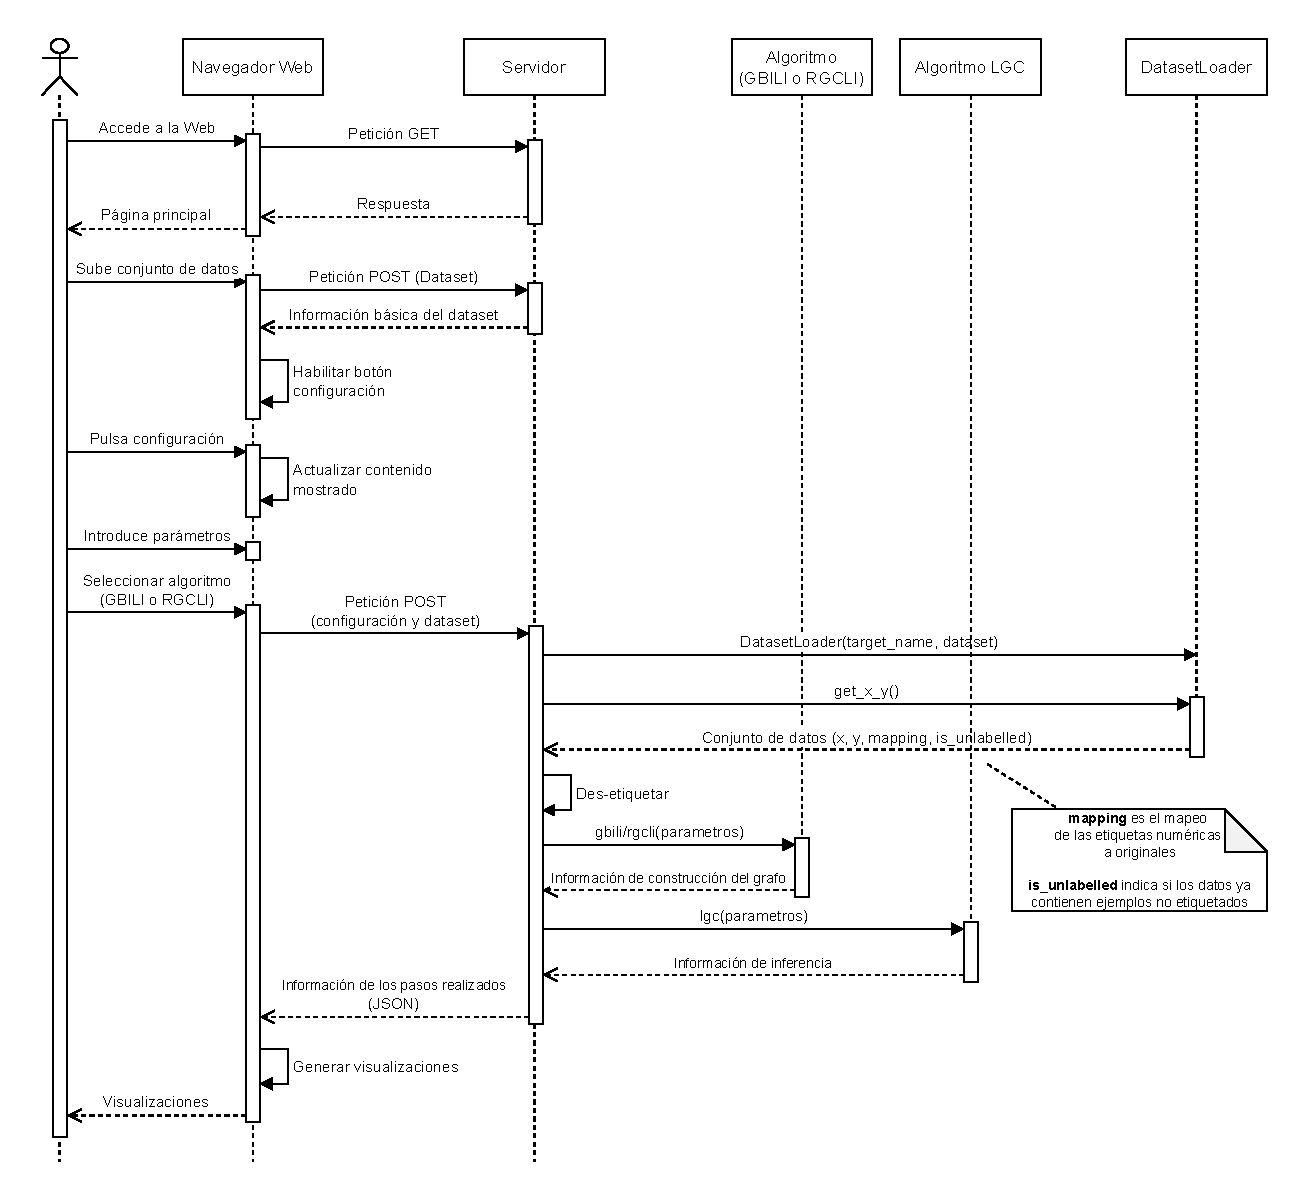
\includegraphics[width=1\textwidth]{figuras/sec.pdf}
		\caption[Diagrama de secuencia]{\textbf{Diagrama de secuencia.}}\label{fig:sec}
\end{figure}

\subsection{Diseño de datos}

En esta sección se describe la información que fluye entre el servidor y el cliente. La figura \ref{fig:sec} representa esa última respuesta del servidor (``Información de los pasos realizados'').

El diseño de la lógica está pensado de tal forma que dependiendo qué algoritmo de construcción de grafo se quiera visualizar, se realiza una petición a una ruta u otra. Esto quiere decir que, salvo la información de los pasos de la construcción (GBILI o RGCLI), el resto es común (el algoritmo de inferencia LGC). El objetivo de ambas rutas es responder con un texto tipo \Gls{json}, que JavaScript es capaz de manejar de forma nativa y directa.


\lstset{
    language=Python,
    basicstyle=\ttfamily\small,
    keywordstyle=\color{blue},
    stringstyle=\color{red},
    commentstyle=\color{green},
    backgroundcolor=\color{white},,
    breaklines=true,
    breakatwhitespace=false,
    showspaces=false,
    showstringspaces=false,
    showtabs=false,
    tabsize=4,
    captionpos=b
}


El aspecto de una respuesta de las rutas es algo parecido a la figura \ref{fig:response}. Siempre existe una entrada que representa los pasos del algoritmo de construcción y otra para el algoritmo de inferencia. Sigue una estructura típica de diccionario con claves y valores. La estructura se organiza por niveles. En el primer nivel se hace referencia al algoritmo, en el segundo se hace referencia a cada paso dentro de un algoritmo y en el tercer nivel se encuentra la información interesante del paso.
En este último caso, es de destacar que siempre se informa de los nodos (los ejemplos en el conjunto de datos), de los enlaces que unen dichos nodos de cada paso (los enlaces de un paso pueden no ser los mismo que otro) e información adicional interesante del paso.

\begin{figure}[H]
    \centering
    \begin{minipage}{0.9\linewidth}
        \begin{center}
            \begin{lstlisting}
                    response = {
                    
                        "gbili": {
                            "PASO X": {
                                "nodes": nodes,
                                "links": link_list,
                                "+INFO": INFO
                            }
                        },
                    
                        "lgc": {
                            "PASO X": {
                                "nodes": nodes,
                                "links": link_list,
                                "+INFO": INFO
                            }
                        }
                    }
                    
                    return jsonify(response)
            \end{lstlisting}
        \end{center}
    \end{minipage}
    \caption{Estructura de la respuesta}
    \label{fig:response}
\end{figure}


\noindent\textbf{\large Pasos de GBILI} \\
Los pasos más relevantes que se han querido mostrar son: construcción de la matriz de distancias, obtención de los vecinos más cercanos, obtención de los vecinos mutuos, conectar vecinos cercanos a puntos etiquetados y el grafo final. Todo estos pasos están descritos en \ref{teoria-gbili} y mostrados en el pseudocódigo \ref{gbili}.

\begin{figure}[h!]
    \centering
    \begin{minipage}{0.9\linewidth}
        \begin{center}
            \begin{lstlisting}
                "gbili": {
                    "dataset": {
                        "nodes": nodes,
                        "links": [],
                        "distance": D.tolist()
                    },
                    "knn": {
                        "nodes": nodes,
                        "links": links_knn,
                        "neighbors": D_argsort.tolist()
                    },
                    "m_knn": {
                        "nodes": nodes,
                        "links": links_m_knn,
                        "mneighbors": m_knn
                    },
                    "semi_graph": {
                        "nodes": nodes,
                        "links": links_semi_graph,
                        "components": [component_membership_semi[i] for i in range(len(X))],
                        "components_with_labeled": list(components_with_labeled)
                    },
                    "graph": {
                        "nodes": nodes,
                        "links": links_graph,
                        "unions": list(unions),
                        "components": [component_membership_graph[i] for i in range(len(X))]
        
                    }
                }
            \end{lstlisting}
        \end{center}
    \end{minipage}
    \caption{Pasos GBILI}
    \label{fig:pasos-gbili}
\end{figure}

\begin{enumerate}
    \item \textit{\textbf{dataset}}: En este paso no existen enlaces todavía, se incluye la matriz de distancias D de cada par de nodos.
    \item \textit{\textbf{knn}}: En este paso, los enlaces representan uniones entre los vecinos más cercanos. Un elemento de la lista de enlaces tiene la forma:\\
    \begin{minipage}{\linewidth}
        \begin{center}
            \begin{lstlisting}
                    {"source": nodo origen, 
                    "target": nodo destino, 
                    "value": fuerza del enlace}
            \end{lstlisting}
        \end{center}
    \end{minipage}
    
    Además, se incluyen esos vecinos más cercanos de cada nodo como una lista (la posición i-ésima contiene los vecinos más cercanos del nodo i). 
    \item \textit{\textbf{m\_knn}}: En este paso, los enlaces representan uniones entre los vecinos más cercanos mutuos. Además, se incluyen esos vecinos más cercanos mutuos de cada nodo como una lista (la posición i-ésima contiene los vecinos más cercanos mutuos del nodo i).
     \item \textit{\textbf{semi\_graph}}: En este paso, los enlaces creados son parte del grafo final. Se incluye también un listado que indica la componente a la que pertenece cada nodo (la posición i-ésima contiene el número de componente a la que pertenece el nodo i). Por último, se construye un listado con las componentes que tienen algún punto etiquetado en ellas.
     \item \textit{\textbf{graph}}: Los enlaces representan el grafo final construido. ``unions'' es una lista de tuplas de dos elementos en la que cada una contiene el número de las dos componentes unidas. Se incluye de nuevo un listado que indica la componente a la que pertenece cada nodo (en el grafo final).
\end{enumerate}

\newpage
\noindent\textbf{\large Información de RGCLI} \\
Para RGCLI, los pasos más relevantes que se han querido mostrar son: construcción de la matriz de distancias, obtención de los vecinos más cercanos, el más cercano etiquetado y el k-ésimo más lejano y, por último, el grafo final construido. Todo estos pasos están descritos en \ref{teoria-rgcli} y mostrados en el pseudocódigo \ref{rgcli}.

\begin{figure}[h!]
    \centering
    \begin{minipage}{0.9\linewidth}
        \begin{center}
            \begin{lstlisting}
                "rgcli": {
                    "dataset": {
                        "nodes": nodes,
                        "links": [],
                        "distance": D.tolist()
                    },
                    "searchknn": {
                        "nodes": nodes,
                        "links": links_knn,
                        "kNN": kNN.tolist(),
                        "L": L.tolist(),
                        "F": F_rgcli.tolist()
                    },
                    "graph": {
                        "nodes": nodes,
                        "links": links_graph
                    }
                }
            \end{lstlisting}
        \end{center}
    \end{minipage}
    \caption{Pasos RGCLI}
    \label{fig:pasos-rgcli}
\end{figure}

\begin{enumerate}
    \item \textit{\textbf{dataset}}: En este paso no existen enlaces todavía, se incluye la matriz de distancias D de cada par de nodos.
    \item \textit{\textbf{searchknn}}: En este paso, los enlaces representan uniones entre los vecinos más cercanos. El formato de la lista de enlaces es el mismo que para GBILI. Además, se incluyen esos vecinos más cercanos mutuos de cada nodo del mismo modo que en GBILI, el etiquetado más cercano de cada nodo y el k-ésimo más lejano.
     \item \textit{\textbf{graph}}: Los enlaces representan el grafo final construido.
\end{enumerate}

\noindent\textbf{\large Información de \Gls{lgc}} \\
Este algoritmo es común para los dos anteriores y los pasos más relevantes que se han querido mostrar son: construcción de afinidad, creación de la matriz S, el proceso iterativo de inferencia y, por último, el etiquetado de los datos. Todo estos pasos están descritos en \ref{teoria-lgc} y mostrados en el pseudocódigo \ref{lgc}.

\begin{figure}[h!]
    \centering
    \begin{minipage}{0.9\linewidth}
        \begin{center}
            \begin{lstlisting}
                "lgc": {
                    "affinity": {
                        "nodes": nodes,
                        "links": links_graph,
                        "F": F.tolist(),
                        "W": W.tolist(),
                    },
                    "S": {
                        "nodes": nodes,
                        "links": links_graph,
                        "D": D_diag.tolist(),
                        "D_sqrt_inv": D_sqrt_inv.tolist(),
                        "S": S.tolist(),
                    },
                    "iteration": {
                        "nodes": nodes,
                        "links": links_graph,
                        "F_history": F_t_history.tolist(),
                        "pred_history": pred_history.tolist()
                    },
                    "labels": {
                        "nodes": nodes_final,
                        "links": links_graph,
                        "F_final": F_t_history[-1].tolist(),
                        "pred_final": pred_history[-1].tolist()
                    }
                }
            \end{lstlisting}
        \end{center}
    \end{minipage}
    \caption{Pasos LGC}
    \label{fig:pasos-lgc}
\end{figure}

Algo común a todos los pasos es que los enlaces representan el grafo final construido (proveniente de unos de los algoritmos anteriores). La demás información se resume en:
\begin{enumerate}
    \item \textit{\textbf{dataset}}: Se incluye la matriz de afinidad (W) y también una matriz de etiquetado similar a \ref{matriz-etiquetado} (F), que representa las etiquetas de cada nodo.
    \item \textit{\textbf{S}}: En este paso se calcula la matriz S (versión normalizada de W). Para su cálculo se utiliza $D$ y $D^{-1/2}$. Se incluyen ambas matrices y la matriz $S$. En realidad, su inclusión solo es por completitud, es interesante ver el formato de esa nueva matriz $D$ (que es diagonal).
    \item \textit{\textbf{iteration}}: Incluye un historial tanto de las etiquetas de cada nodo ``pred\_history'' (una lista de listas de una dimensión) como de la matriz de etiquetado ``F\_history'' (una lista de matrices donde cada una es como \ref{matriz-etiquetado} y se tiene una por cada iteración de LGC).
    \item \textit{\textbf{labels}}: Incluye la última lista de ``pred\_history'' (``pred\_final'') y la última matriz de etiquetado ``F\_final'' (``F\_final'').
\end{enumerate}

\begin{singlespace}
\begin{footnotesize}
\begin{twocolumn}
\bibdata{bibliografia}
\bibliography{bibliografia}
\addcontentsline{toc}{chapter}{Bibliografía}
\end{twocolumn}
\end{footnotesize}
\end{singlespace}

\end{document}
